\chapter{The ATLAS Detector}
\label{chap:ATLAS}

The \ac{ATLAS} detector is a cylindrical general purpose particle detector designed to measure the products of $\sqrt{s} = 14 \TeV$ proton-proton collisions at the \ac{LHC}. It consists of three major sub-detectors: closest to the beamline is the the Inner Detector (ID), which measures the trajectories of charge particles, followed by the Calorimeters, which measure the energies of electromagnetic and hadronically interacting particles, and finally the Muon Spectrometer (MS) which measures the trajectories of muons. The \ac{ID} is surrounded by a super conducting solenoid that provides a uniform $2$ T magnetic field, enabling measurement of particles' charge and momentum. A toroidal magnet surrounds \ac{MS}, for charge and momentum measurements of muons. In general, each subdetector consists of a barrel detector parallel to the beamline and perpendicular end-cap detectors on either end of the barrel detectors. \cite{atlas-overview}

A schematic of the \ac{ATLAS} detector is shown in \autoref{fig:atlas-schematic}.


%https://atlas.cern/discover/detector
\begin{figure}[!h]
\centering
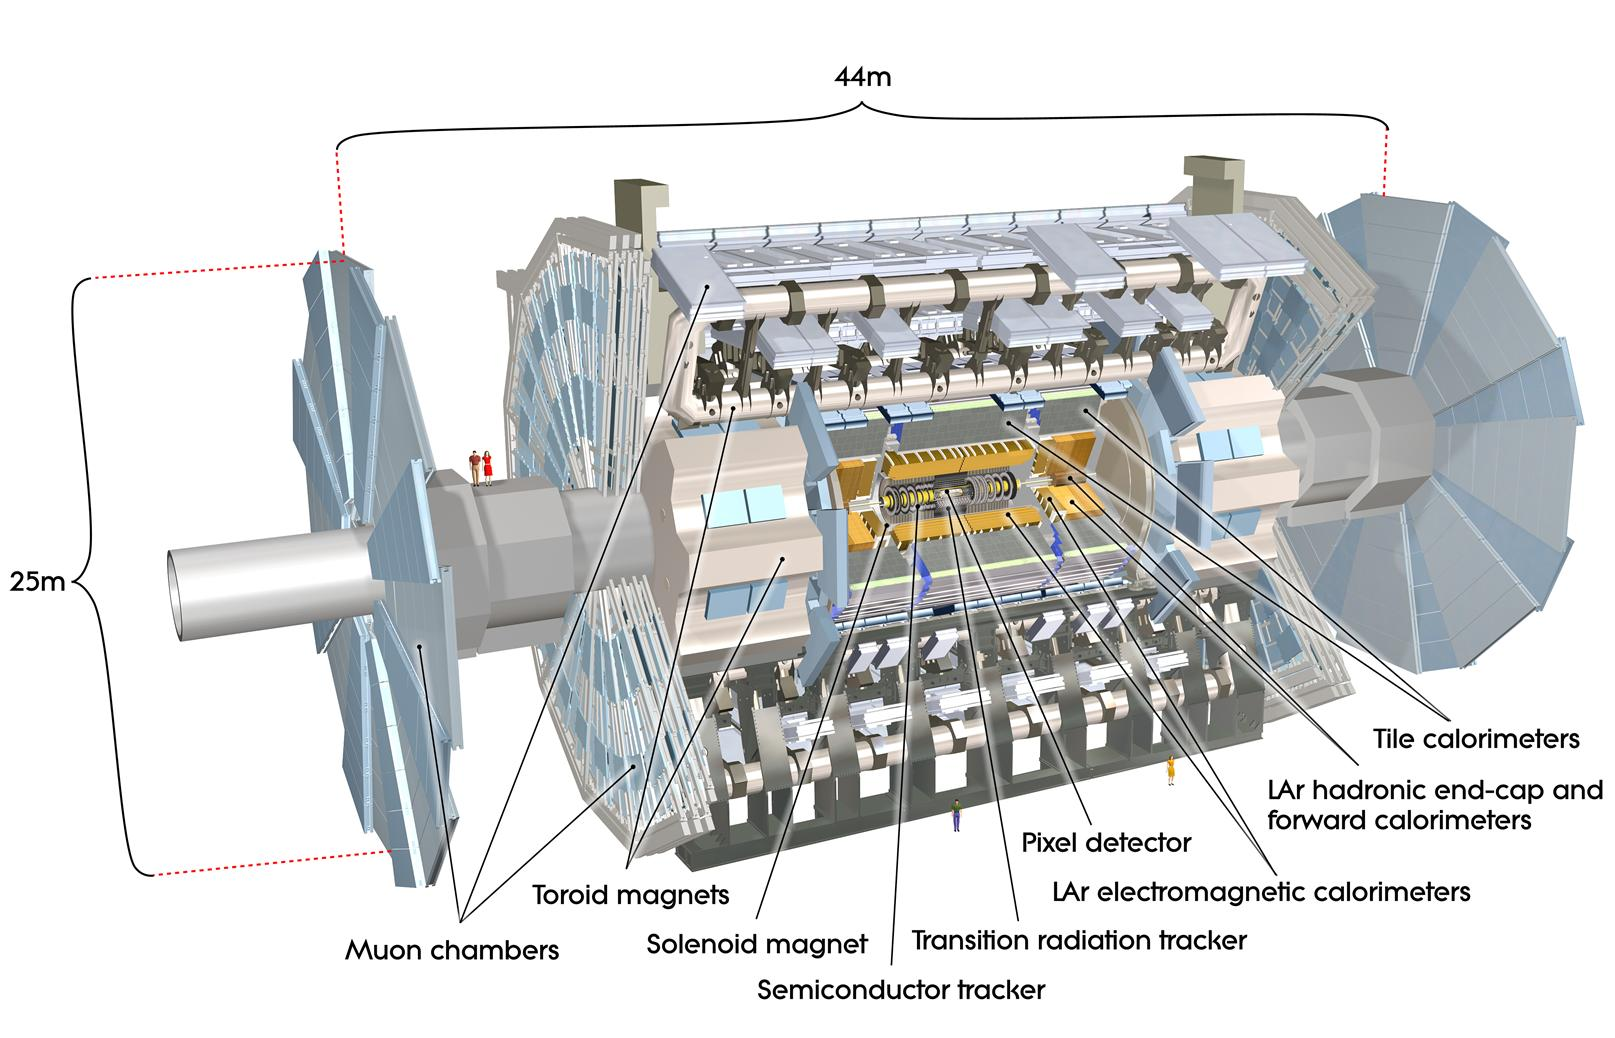
\includegraphics[width=.7\textwidth]{figures/Detector/atlas-schematic.jpg}
\caption{A diagram of the \ac{ATLAS} detector. The dimensions, subdetectors, and magnet systems are labeled. }
\label{fig:atlas-schematic}
\end{figure}

\section{Coordinate System}
\ac{ATLAS} uses a Cartesian right-handed coordinate system. The $z$-axis points along the beampipe, where $+z$ points counter-clockwise. The transverse plane, the $y$-axis and $x$-axis, points upward and toward the center of the \ac{LHC} ring, respectively. The detector is built with with symmetry across the origin in in $z$, as well as with rotational symmetry in the transverse plane. The origin is the $pp$ collision point, generally somewhere near $x=y=z=0$. The $+z$ side of the detector is referred to as the A-side, and $-z$ as the C-side. 

Cylindrical coordinates are generally used to describe the \ac{ATLAS} detector, where $\phi$ measures the angle in the $x-y$ plane around the beam axis, and $\theta$ the angle from the $z$ axis. $\phi$ is positive for positive $y$. 

A given particle's momentum in the $z$ direction is not known, but since the beams collide head on along the $z$-axis, its transverse momentum must be $0$, so it is advantageous to define spatial variables independent of $z$ momentum. Thus, instead of $\theta$, \emph{pseudorapidity} is used to describe angle from the $z$ axis. $\eta$ is defined as
\begin{equation}
\eta = - \textrm{ln}(\textrm{tan}\frac{\theta}{2}) 
\end{equation}
Particles perpendicular to the $z$ axis have $\eta = 0$, while those parallel to the beamline have $\eta \rightarrow \infty$. The particle distribution from \ac{LHC} collisions is roughly uniform in $\eta$ and $\eta$ is invariant under Lorentz boosts assuming massless particles.

Angular distances between objects is described using $\Delta R = \sqrt{\Delta \eta ^2 + \Delta \phi ^2}$ and the radial distance from the origin in the $x-y$ plane is denoted $R$. 

A particle's momentum will generally be described in terms of its \pT, its momentum in the transverse direction. A particle's $3$-vector is described by $(\pt, \eta, \phi)$, which are all invariant under boosts in $z$ assuming the particle can be considered massless.


%USED ATLAS-overview.pdf
\section{Inner Detector}
The Inner Detector measures the trajectories of charged particles resulting from \ac{LHC} collisions. The \ac{ID} covers the region with $|\eta| < 2.5$, measuring approximately $1000$ particles per bunch crossing. In order to achieve the momentum and vertex resolution required to achieve \ac{ATLAS}'s physics goals three subdetectors are used: the Pixel detector, the \ac{SCT}, and the \ac{TRT}. The Pixel and \ac{SCT} detectors are used for high granularity precision tracking and the \ac{TRT} is used to distinguish electrons from low-mass hadrons like pions. All of this is immersed in a $2$T magnetic field, bending the trajectories of charged particles in proportion to their momentum in the $\phi$ direction.

The \pt resolution of the \ac{ID} scales with track \pt. Higher \pt tracks are less curved, so the measurement resolution is worse. In the \ac{ATLAS} \ac{ID}, the \pt resolution  $0.05\% \times \pt$ with a $1\%$ constant term. The constant term describes measurement uncertainties that do not scale with momentum or energy, such as material imperfections, non-uniform detector response, or other constant measurement issues and is added in quadrature ($\oplus$) with the stochastic term.

The combination of the three trackers with radii ranging from 32.33 mm to 1082 mm enable robust and precise pattern recognition of all charged particles that pass through the detector. The Pixel and \ac{SCT} detectors provide secondary vertexing and impact parameter measurement and vertexing for heavy-flavor jet and $\tau$-lepton tagging. The \ac{TRT} has lower precision per point, but measures a longer track and contributes significantly to momentum measurements.


A sketch of the \ac{ID} can be seen in \autoref{fig:atlas-id} and a detailed schematic of the various subdetectors is shown in \autoref{fig:atlas-id-layers}. 


%https://cds.cern.ch/images/CERN-GE-0803014-01/file?size=medium
\begin{figure}[!h]
\centering
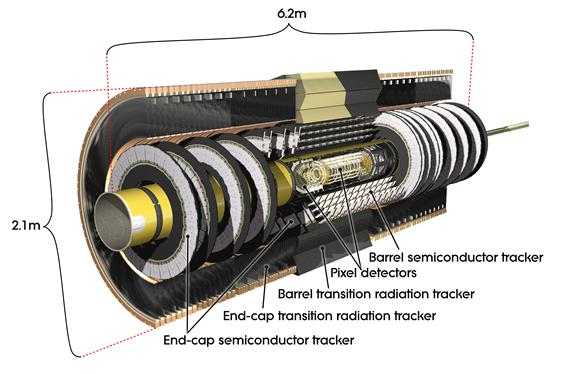
\includegraphics[width=.7\textwidth]{figures/Detector/atlas-ID.jpg}
\caption{A diagram of the \ac{ATLAS} \ac{ID} with the major subsystems labeled. The Pixel and \ac{SCT} are of particular importance for this analysis.}
\label{fig:atlas-id}
\end{figure}

%https://www.researchgate.net/publication/325643426/figure/fig8/AS:669532737769482@1536640452588/Segment-of-the-ATLAS-inner-detector-showing-the-tracker-layers-The-silicon-strip.ppm
\begin{figure}[!h]
\centering
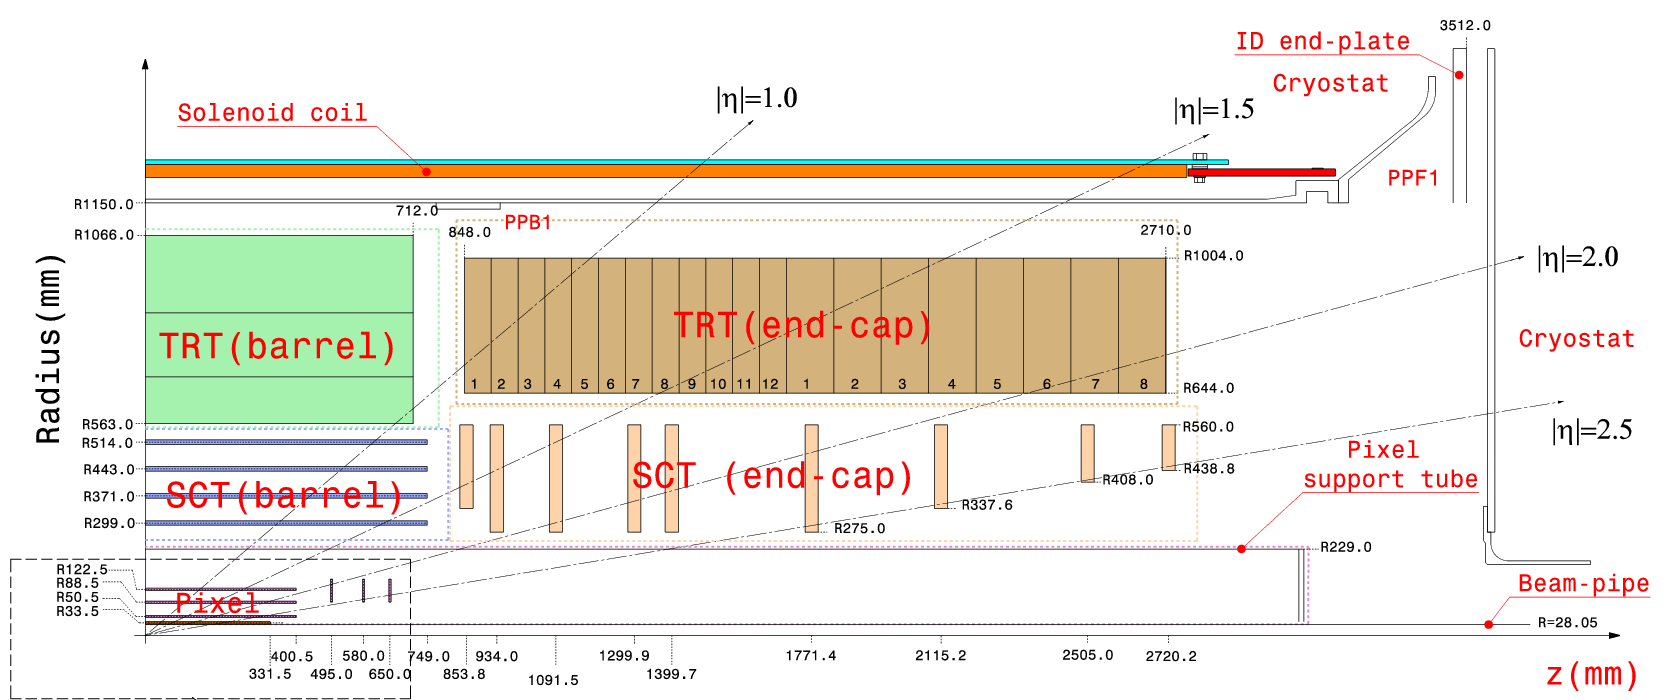
\includegraphics[width=.7\textwidth]{figures/Detector/atlas-id-layers.png}
\caption{A schematic of the \ac{ATLAS} \ac{ID} shown in the $R-z$ plane. \cite{id-cutaway}}
\label{fig:atlas-id-layers}
\end{figure}


The two innermost detectors, the Pixel and \ac{SCT} detectors, are made of silicon, which is the preferred tracking medium of particle physics. The \ac{ATLAS} pixels are n-type semiconductors, which have added impurities to increase the number of potential electron charge carriers. A voltage is applied, 150-600V in the Pixel detector.  When a charged particle interacts with a silicon detector layer, electron-hole pairs are created and these pairs drift toward the readout chips in the magnetic field. If enough of these pairs are created such that the signal becomes greater than a pre-specified noise threshold, the signal is readout as a \emph{hit}. A particle must have 3.6 eV to induce about 80 electron-hole pairs per $\mu$m. Pixels provide a high signal-to-noise ratio, and so are preferred in regions where high occupancy is possible, like the region closest to the beamline. \cite{silicon} 

\subsection{The Pixel Detector}

The Pixel detector is the closest to the beam and has the highest granularity. The detector is composed of pixels arranged parallel to the beam axis in concentric cylindrical layers in the barrel and perpendicular to the beam axis on disks in the endcap regions. The current Pixel detector consists of the Run 1 detector with the \ac{IBL} installed closer to the beam pipe. 

The Run 1 Pixel detector has 3 concentric cylindrical layers in the barrel and 3 disks in the endcap. It is composed of 1744 pixel sensors, each with 47,232 pixels. Each pixel is identical has minimum size of $R\phi \times z = 50 \times 400~\um^{2}$ (increasing to $R\phi \times z = 50 \times 600~\um^{2}$ near a readout chip). In the barrel, they give track resolutions of $10~\um$ in $R\phi$ and $115~\um$ in $z$, and in the endcaps they have accuracy of $10~\um$ in $R-\phi$ and $115~\um$ in $R$ and the detector has 80.4 million pixels, each with its own readout channel. 

The \ac{IBL} is the inner most Pixel layer installed for Run 2 33.2 mm away from a new, narrower beampipe. A closer detector layer enables better impact parameter resolution as well as providing extra radiation shielding for the former closest Pixel layer (called the B-layer). The \ac{IBL} is composed of 12 million smaller pixels, $R\phi \times z = 50 \times 250~\um$, assembled on 14 staves, with a resolution of $8~\um$ in $R\phi$ and $40~\um$ in $z$.



\subsection{The Silicon Microstrip Tracker}
A particle moving through the \ac{SCT} crosses 4 bilayers of the detector creating 4 hit measurements as it interacts with 8 layers of material. A  bilayer is composed of 2 stereostrips composed of two thin layers of silicon: one parallel to the beam axis (measuring $R\phi$) and the other rotated by 40 mrad. The combination of the stereostrips in the bilayer gives a 3-dimensional measurement. In the barrel, they are arranged in concentric cylinders parallel to the $z$ axis and in the end caps, they are arranged on 9 disks per side. The strips are 12 cm long and $80 \mu\textrm{m}$ thick.

Less precise than the Pixels, they have accuracy of $17 \mu \textrm{m}$ in $R-\phi$ and $580 \mu \textrm{m}$ in $z$ in the barrel region, and in the endcaps they have resolution of $17 \mu \textrm{m}$ in $R-\phi$ and $580 \mu \textrm{m}$ in $R$. The use of strips instead of pixels reduces the number of readout channels as well as the cost: there are 15,192 sensors each with 768 strips with an applied voltage of 150-300V and 6.3 million readout channels.
 

\subsection{The Transition Radiation Tracker}
The \ac{TRT} is straw-tube tracker that extends the tracking volume by almost 500 mm without the cost of that much additional silicon. The tubes have a diameter of 4mm and made of Kapton and carbon fibers. They are filled with a gas mixture (70\% Xe, 27\% CO$_{2}$, and 3\% O$_{2}$) and a 31 $\mu$m diameter gold-plated tungsten wire. The wires are divided into two halves about $\eta = 0$. In the barrel, the 52,544 straws are parallel to the beam axis and 144 cm long. In the endcaps, 122,880 37 cm long straws are arranged radially in wheels. The \ac{TRT} 351,000 readout channels, much fewer than the silicon detectors.

When a charged particle passes through the tube, the gas is ionized and the resulting free electrons drift toward the wire where they are amplified then readout. A particle passing through the \ac{TRT} typically leaves 36 hits. The \ac{TRT} only provides $R\phi$ measurements with an accuracy of $130~\um$ per straw. However, it has the advantage that its radius improves the momentum resolution, and it  can provide ns-level timing information.


\subsection{Solenoid Magnet}

The central solenoid surrounds the \ac{ID} and provides a uniform $2~\textrm{T}$ field that bends the trajectories of charged particles. The transverse momentum of the particle can be inferred from its radius of curvature, $R$, in the $x-y$ plane using the equation $p_{T} = qBR$, where $q$ is the charge of the particle and $B$ the magnetic field in the $z$ direction.

However, the placement of the solenoid between the \ac{ID} and calorimeters necessitates careful design choices so that all of a given particle's energy is still measured by the calorimeters. The solenoid only contributes about $0.66$ \emph{radiation lengths}, the mean distance in which an electron loses all but $\frac{1}{e}$ of its energy. In order to achieve this, the solenoid and \ac{EM} calorimeter share a vacuum vessel, eliminating the need for two vacuum walls. It is made of Al-stabilised NbTi superconductor which allows a high electric field to be achieved ($7.730 \textrm{kA}$) while optimizing the thickness of the coil. The solenoid has an axial length of $5.8~\textrm{m}$ and radial thickness of $100~ \textrm{cm}$ and it operates at a temperature of $4.5~\textrm{K}$. 


\section{Calorimeters}

The \ac{ATLAS} calorimeters measure the energy of particles which interact via electromagnetic and hadronic interactions. The calorimeter system is composed of \ac{EM}, hadronic, and forward calorimeters. While they use a variety of different technologies to measure energies, they are all sampling calorimeters composed of alternating active and absorbing layers. Particles shower in absorbing layers and the showers are measured in the active layers. The actual energy of each particle is not measured due to energy loss in the absorbing layers. The size of each calorimeter is set by its radiation length or nuclear interaction length such that the calorimeter absorbs all of given particle's energy by the time it reaches the end of the calorimeter. The only Standard Model particles that should escape the calorimeters are neutrinos and muons; neutrinos do not interact with the material of any of the detectors, and muons are too heavy to be stopped by the EM calorimeter. Unlike the tracker, the energy resolution of a calorimeter increases with increasing energy due to the increased signal generated.  A schematic of the \ac{ATLAS} calorimeters can be seen in \autoref{fig:atlas-calos}.


%https://arxiv.org/pdf/1603.02934.pdf
\begin{figure}[!h]
\centering
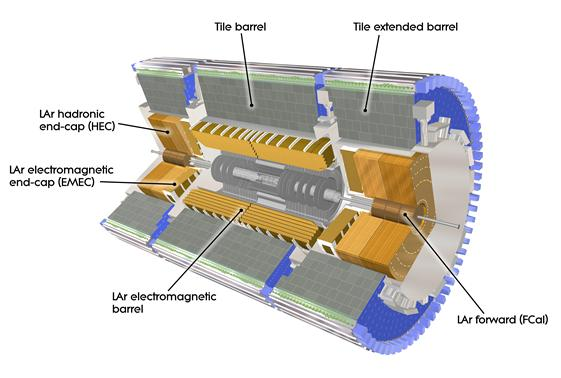
\includegraphics[width=.7\textwidth]{figures/Detector/atlas-calorimeters.jpg}
\caption{A diagram of the \ac{ATLAS} calorimeters with the major subsystems labeled. The \ac{EM} calorimeter is of particular importance for this analysis. \cite{calorimeters}}
\label{fig:atlas-calos}
\end{figure}


\subsection{Electromagnetic Calorimeter}

The Liquid Argon (LAr) Electromagnetic (EM) calorimeter is the innermost calorimeter and gives excellent energy and position resolution \cite{calorimeters}. It is composed of barrel ($|\eta| < 1.5$) and end-cap ($1.4 < |\eta| < 3.2$) components. Both components use a lead absorber with liquid argon active material. The layers of the calorimeter have an accordion shape (shown in \autoref{fig:atlas-lar}), which allows for multiple absorbing layers without any gaps between them, as well as complete $\phi$ symmetry. The first layer has finer segmentation in $\eta$ to allow for more precise angular measurements of photons (which do not produce an \ac{ID} track). The thickness of the absorbing plates varies as a function of $\eta$ to optimize energy resolution. A liquid argon active presampler is placed before the accordion layers in the region with $|\eta| < 1.8$ to correct for energy loss upstream of the calorimeter. The whole calorimeter is about 22 radiation lengths wide and gives energy resolution of $10\%/\sqrt{E} \oplus 0.7\%$

%https://www.researchgate.net/profile/Denis_Oliveira_Damazio/publication/229849719/figure/fig2/AS:667635272413188@1536188061121/Calorimeter-cells-for-different-layers-left-Note-the-very-fine-segmentation-in-the_Q320.jpg
\begin{figure}[!h]
\centering
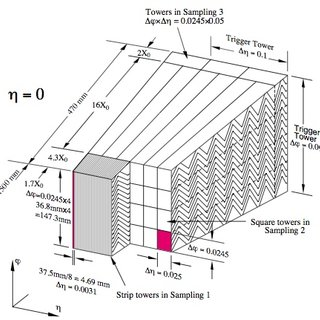
\includegraphics[width=.6\textwidth]{figures/Detector/lar.jpg}
\caption{A diagram of the \ac{ATLAS} \ac{EM} \ac{LAr} calorimeter. It has a unique shape in order to provide precision position and energy resolution.}
\label{fig:atlas-lar}
\end{figure}


\subsection{Hadronic Calorimeter}

The hadronic calorimeter surrounds the \ac{EM} calorimeter also within $|\eta| < 3.2$. The barrel region ($|\eta| < 1.7$) is made of steel absorbers with active material of scintillating tiles. Here, the calorimeter is about $2$ m long in the radial direction and covers about $8$ interaction lengths. The Hadronic End-cap Calorimeters cover the region $1.5 < |\eta| < 3.2$ with a copper absorber and liquid argon active material.


The hadronic calorimeter has an energy resolution of  $50\%/\sqrt{E} \oplus 3\%$. 

\subsection{Forward Calorimeter}
The \ac{FCAL} is measures  both \ac{EM} and hadronic energy and extends coverage to $3.1 < |\eta| < 4.9$. The detector uses liquid argon as its active material with copper (for \ac{EM} activity) and tungsten (for hadronic activity) absorbers. It is about $10$ interaction lengths deep and also serves to add some shielding to the \ac{MS}. The energy resolution of the \ac{FCAL} is $100\%/\sqrt{E} \oplus 10\%$.


\section{Muon Spectrometer}
The Muon Spectrometer is the outermost subdetector and designed to detect and measure the momenta of muons, which are too massive to be stopped by the EM calorimeter and do not interact strongly. This is achieved using a toroidal magnet system that deflects muons as they pass through through  high-precision tracking chambers and separate trigger chambers. The magnetic field points in the $\eta$ direction, orthogonal to the muon's direction of motion. The detector as well as the toroid system has discrete rotational symmetry in $\phi$.

The \ac{MS} can measure muons with $|\eta| < 2.4$ and $3 \GeV < {\pt}_{\mu} < 10 \TeV$. The main performance goal is to provide a stand-alone (independent of the \ac{ID}) momentum resolution of $10\%$ at $\pT > 1 \TeV$; a particle moving with $\pt = 1 \TeV$ has a \emph{sagitta} (see \autoref{fig:ms-sagitta}) of $500~\um$ that needs to be measured with a resolution of $<50\mu\textrm{m}$. Even at 3\TeV, the \ac{MS} has good momentum resolution and is still able identify the charge of the particle based on its bending direction. Furthermore, the triggering chambers have timing resolution of $1.5-4 \textrm{ns}$.  

\begin{figure}[!h]
\centering
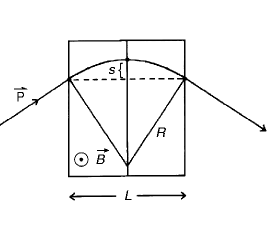
\includegraphics[width=.6\textwidth]{figures/Detector/ms-sagitta.png}
\caption{The trajectory of a particle in a magnetic field (``B''). The particle's sagitta, labeled ``s'' is the bending distance in the direction perpendicular to the magnetic field. The direction of the bending is dictated by the charge of the particle. The higher the momentum of a particle, the smaller the sagitta. \cite{particledetectors-springer}}
\label{fig:ms-sagitta}
\end{figure}


Monitored Drift Tubes (MDTs) are used for precision tracking in the $\eta$ coordinate (the bending direction of the toroids) in the range $|\eta| < 2.7$, except in the inner most layer where the \ac{MDT}s extend only to $|\eta| < 2.0$ and Cathode-Strip Chambers (CSCs) cover the region $2.0 < |\eta| < 2.7$. Triggering and $\phi$ measurements are provided by Resistive Plate Chambers (RPCs) in the range $|\eta| < 1.05$ and Thin Gap Chambers (TGCs) in $1.05 |\eta| < 2.7$. The detector chambers are arranged in concentric cylindrical shells around the beam axis at radii of about 5 m, 7.5 m and 10 m in the barrel, and on wheels perpendicular to the beam axis at distances of about 7.4 m, 10.8 m, 14 m, and 21.5 m from the interaction point. There is a gap in detector coverage around $|\eta| < 0.1$ for detector access for service work. Schematics of the \ac{MS} can be seen in \autoref{fig:atlas-ms}.  

\begin{figure}[!h]
\centering
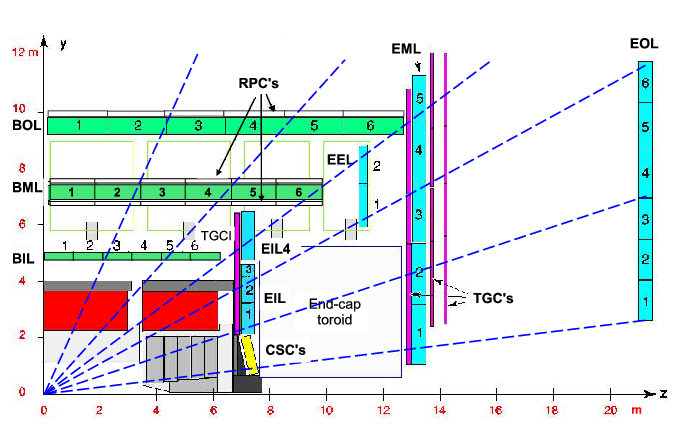
\includegraphics[width=.6\textwidth]{figures/Detector/atlas-ms.png}
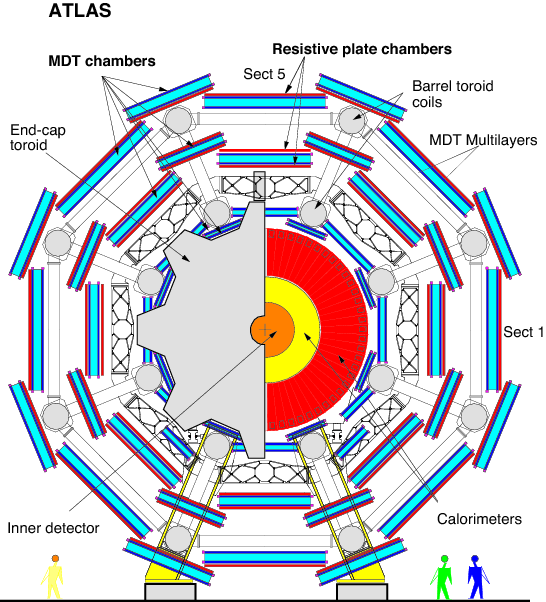
\includegraphics[width=.3\textwidth]{figures/Detector/mdt-phi.png}
\caption{A diagram of the \ac{ATLAS} \ac{MS} in the $r-z$ (left) plane and a $\phi$ cross section of the barrel region. On the left, the barrel \ac{MDT} are shown in green and the \ac{RPC} shown in black. In the end-caps, the \ac{MDT} are shown in blue and the \ac{TGC} shown in purple. On the right, the concentric cyclindrical layers of \ac{MDT}s are shown: 8 small chambers and 8 large chambers. The diameter is 20m at its widest. \cite{ms-vertices}}
\label{fig:atlas-ms}
\end{figure}


While the \ac{MDT}s give extremely precise measurements of muon directions, they cannot be used in isolation for the physics goals of \ac{ATLAS}. First, they are finely segmented in $\eta$, the bending direction of the muons, enabling the high momentum resolution. However, in $\phi$, their resolution is as good as the length of the tube, several meters long or $\approx 0.1$ in $\phi$. Additionally, being drift tubes, their readout is very slow and cannot be used for triggering, which requires a quick response. Thus, \ac{RPC}s (in the barrel) and \ac{TGC}s (in the endcaps) complement the \ac{MDT}s for triggering and \ac{CSC}s complement the \ac{MDT}s in the forward region (where the particle flux is the highest) to provide better 2-dimensional position measurements. A comparison of the resolution of the different detectors of the \ac{MS} can be seen in \autoref{tab:ms-parts}. 

\begin{table}[htb]
\begin{center}
\begin{tabular}{ccccc}
detector    & function & z/R resolution & $\phi$ resolution & time resolution \\
 \hline
  \ac{MDT}  &  tracking   &  35 \um (z)  & 2.5-5 m  & $<$ 700 ns \\
  \ac{CSC}  &  tracking   &  30 \um (R)  & 5 mm     & 7 ns   \\
  \ac{RPC}  &  triggering &  10 mm  (z)  & 10 mm    & 1.5 ns  \\
  \ac{TGC}  &  triggering &  2-6 mm (R)  & 3-7 mm   & 4 ns  \\
\hline
\end{tabular}
\caption{Resolutions of the various parts of the \ac{MS}. The endcap detectors (\ac{CSC}s and \ac{TGC}s) give resolution in R while the barrel detectors (\ac{MDT}s and \ac{RPC}s) give resolution in z. The various pieces of the \ac{MS} enable 2 dimensional precision measurement as well as measurements to be used in the trigger.}
\label{tab:ms-parts}
\end{center}
\end{table}

\subsection{Monitored Drift Tubes and Cathode-Strip Chambers}

The fundamental unit of the \ac{MDT} chambers are 30 mm diameter pressurized drift tubes. Each drift tube is filled with Ar/CO$_{2}$ gas and a 50 \um~ diameter tungsten-rhenium wire. When a muon passes through the tube, it ionizes the atoms in the gas. Ionized electrons travel along the electric field in the tube until they reach the positively charged wire. The location of the electrons along the wire give a position measurement. \ac{MDT} hits are referred to as \emph{precision hits}. The time of arrival of the first charges at the wire determine the radius of the drift-circle, seen in \autoref{fig:ms-drift}. If the muon itself passes close to the wire during its trajectory it can induce a signal in the wire, so a dead time is specified before the detector readout. The spatial resolution of a single drift tube is 80 \um. 

Each \ac{MDT} chamber consists of two multilayers of drift tubes separated by a mechanical spacer. The inner chambers, where the highest performance is required, a multilayer is composed of four layers of drift tubes (increasing the resolution to 30 \um), while in the middle and outer chambers multilayers are composed of three layers (increasing the resolution to 35 \um). The combination of the three chambers gives the required sagitta resolution with about 15 measurements per muon. There are 1150 \ac{MDT} chambers with 354,000 drift tubes. To achieve the required momentum resolution, the tubes must not bend more than 100 \um, a significant challenge against gravity. The tubes are held in tension and carefully calibrated and monitored to achieve a maximum bending of 20 \um. 

The \ac{CSC}s are multiwire proportional chambers with anode wires oriented radially. The wires are held between two cathodes: one segmented with strips perpendicular to the wires giving a precision measurement in the bending plane ($\eta$) of with resolution of 40~\um~ and the other segmented parallel to the wire, giving a transverse ($\phi$) measurement with 5 mm resolution. The signals from the wires are not read out, rather a position is obtained by measuring the relative charge deposited on neighboring strips. The \ac{CSC}s are segmented into chambers in $\phi$, each consisting of four layers, resulting in four measurements per muon.


\subsubsection{MDT Timing}
\label{sec:mdt-timing}
The readout of the \ac{MDT}s also gives a profile of the hits that compose the signal in time, seen in \autoref{fig:ms-t0fit}. The peak of the distribution, $t_{0}$, measures the time the signal began with respect to $t=0$, the time of the $pp$ interaction measured by the \ac{ATLAS} clock. The end of the signal, $t_{\text{max}}$, is the maximum drift time. In a perfectly calibrated detector, the $t_{0}$ measurement is Gaussian about $t_{0} = 0$ with a width of about 3 ns. 



\begin{figure}[htbp]
\centering
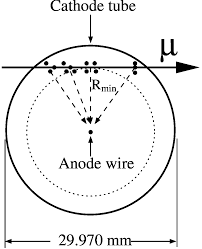
\includegraphics[width=.4\textwidth]{figures/Detector/ms-drift.png}
\caption{A sketch of a muon passing through a cross section of an \ac{MDT}. \cite{atlas-overview}}
\label{fig:ms-drift}
\end{figure}

\begin{figure}[htbp]
\centering
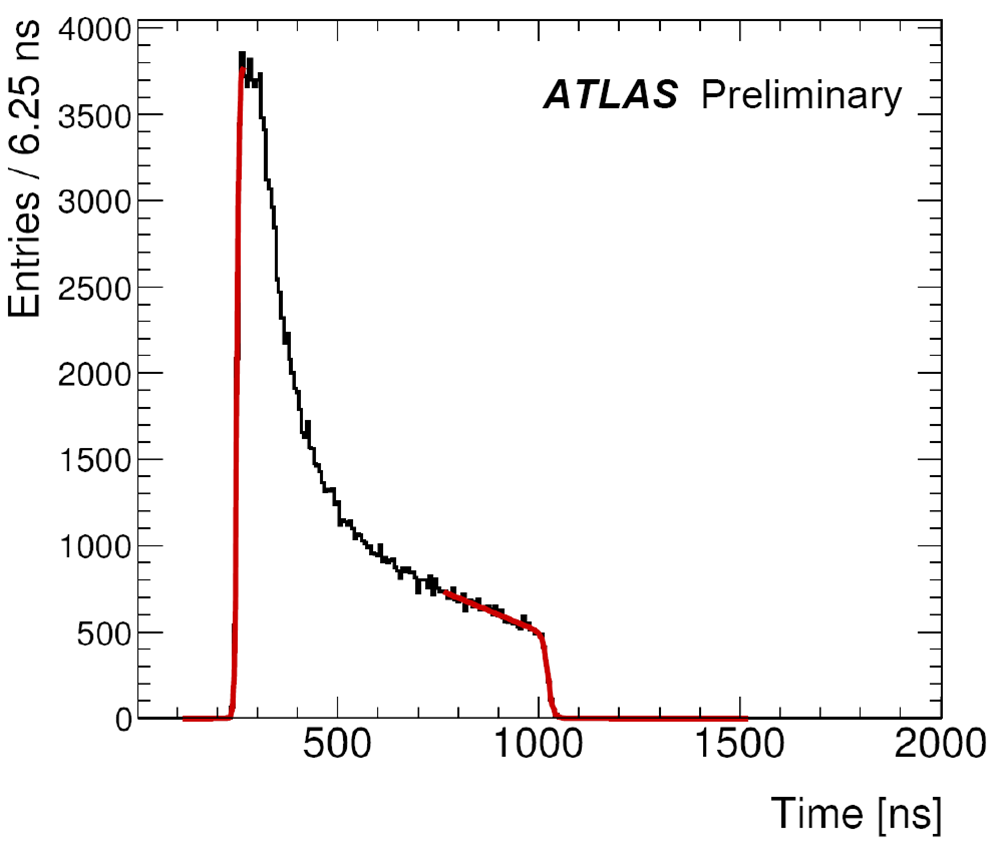
\includegraphics[width=.5\textwidth]{figures/Detector/mdt-t0.png}
\caption{A distribution of \ac{MDT} time measurements. The $t_{0}$ is the time between 0 and the peak of the distribution, shown by the leftmost red line. The rightmost red line indicates $t_{\textrm{max}}$, the end of the \ac{MDT} signal. \cite{muon-public}}
\label{fig:ms-t0fit}
\end{figure}




\subsection{Resistive Plate Chambers and Thin Gap Chambers}

The trigger chambers must provide transverse momentum resolution in the barrel and endcaps over the full $\phi$ range; have time resolution such that detector information can be matched to the correct bunch crossing; be robust against photon and neutron backgrounds in the experimental cavern; and provide a $\phi$ measurement to complement the \ac{MDT} $\eta$ measurement.


In the barrel, \ac{RPC}s are used to achieve these goals. An \ac{RPC} is a parallel plate detector composed of two phenolic-melaminic plastic laminate plates 2 mm apart filled with C$_{2}$H$_{2}$F$_{4}$ gas and with a 4.9 kV/mm field between them. When a muon passes through the detector, it ionizes the atoms in the gas, the ionized electrons further ionize other atoms, creating an avalanche. Both sides of the chamber are readout and they have perpendicular readout strips, giving both $z$ and $\phi$ measurements. The \ac{RPC} are arranged into chambers of two detector layers each (giving two measurements per chamber) and positioned above or below each \ac{MDT} chamber.

In the endcaps, multiwire proportional chamber \ac{TGC}s are used. They work very similarly to the \ac{CSC}s, with perpendicular anode wires and cathode strips, but the unit is more compact, giving the requisite increase in speed. Multiwire proportional chambers are ideal for the endcaps of the \ac{MS} because they have an extremely granular readout, which allows them to deal with the inhomogeneity of the magnetic field in the transition region.


\subsection{Toroid Magnets}

The toroid magnet system, composed of a barrel and two end-caps, provides a toroidal magnetic field of $0.5~\textrm{T}$ and $1~\textrm{T}$ for the barrel ($|\eta| < 1.4$) and end-cap ($1.6 <|\eta| < 2.7$) regions of the \ac{MS}. In the transition region ($1.4 < |\eta| < 1.6$) muons are bent by a combination of the two fields resulting in an extremely heterogeneous field making accurate measurement challenging. This inhomogeneity results in geometric regions where the muon trajectories are not bent at all, mimicking a high \pt muon, adding challenges for triggering on high \pt muons in this region. The toroid is much larger than the solenoid, $25.3 \textrm{m}$ long and $10 \textrm{m}$ in radial width, but also operates at a temperature of $4.5 \textrm{K}$. All three toroid magnets are made of Al-stabilized Nb/Ti/Cu conductor. They have an air-core structure, which gives them a strong bending power over a large volume while minimizing material that could induce any additional scattering. 


\section{Particles in ATLAS}
All of the \ac{ATLAS} subdetectors are used in combination to identify particles. Charged particles interact with the \ac{ID} resulting in hits to be reconstructed into tracks. A track that points to a cluster in one of the calorimeters indicates the kind of charged particle that made the track, and a cluster without an associated track indicates a neutral particle. The calorimeters are designed such that they absorb all of the energy of a particle and particles measured by the \ac{EM} caloriemter should not enter the hadronic calorimeter, and hadronic particles should not enter the \ac{MS}. Muons have minimal interactions with the calorimeters, but do leave a track in both the \ac{ID} and \ac{MS}. The only \ac{SM} particle that escapes the detector entirely is a neutrino. An undetected particle, like an \ac{SM} $\nu$ or some \ac{BSM} particle, could be seen as an imbalance in transverse momentum referred to as \ac{MET}. The transverse momenta of all particles should sum to zero in order to conserve momentum, so any non-zero sum indicates an undetected particle.


\begin{figure}[htbp]
\centering
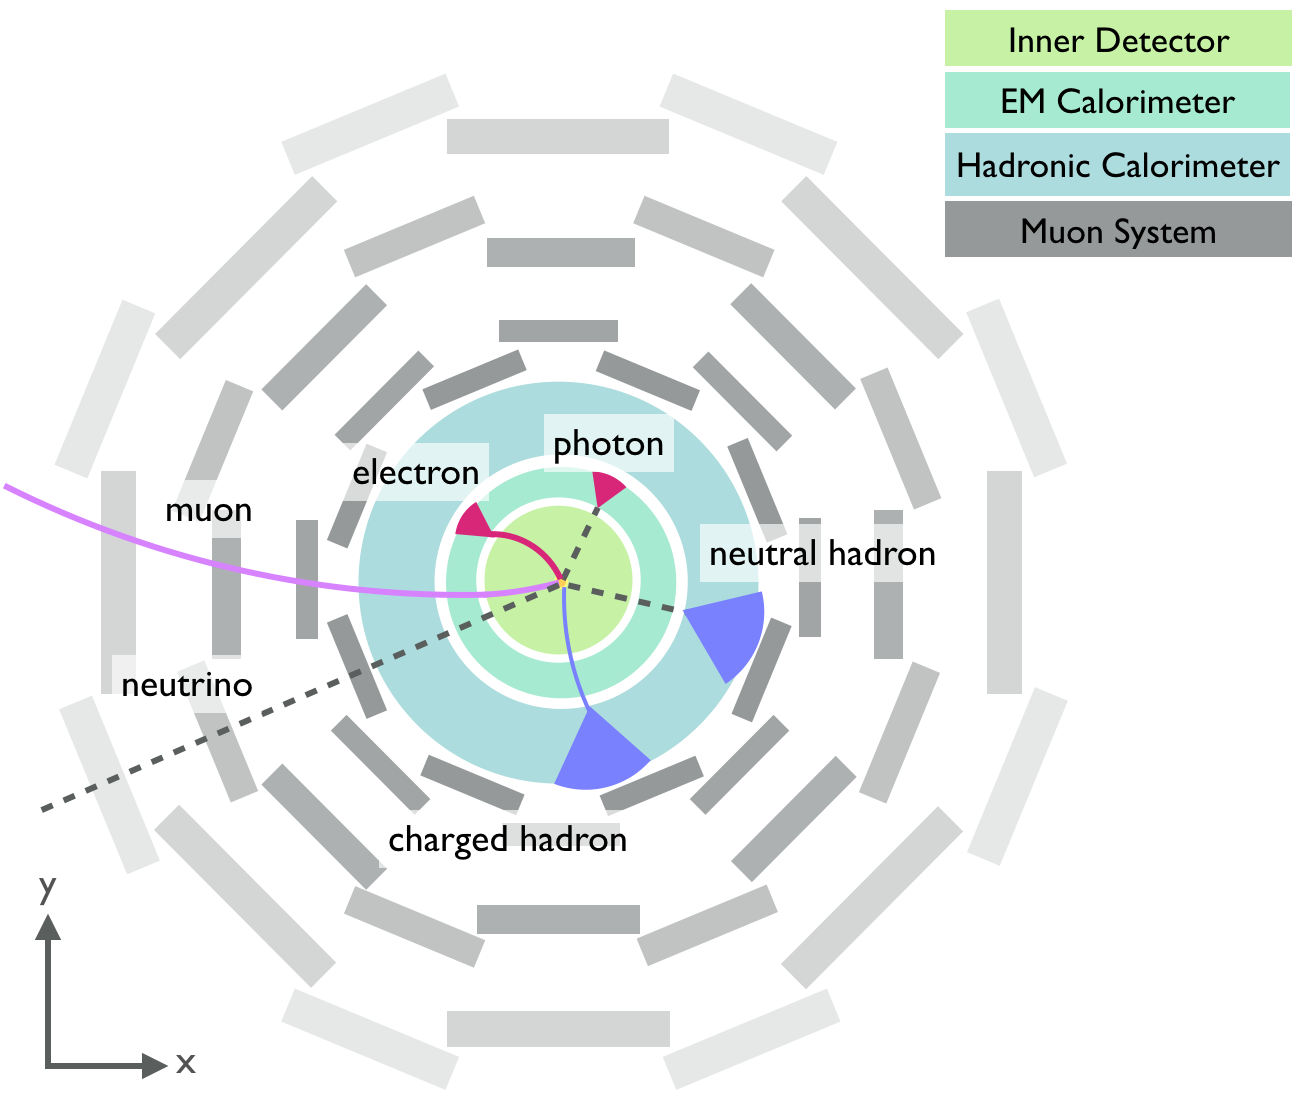
\includegraphics[width=.6\textwidth]{figures/Detector/particle-doodle.png}
\caption{A schematic of the signatures of Standard Model particles in the \ac{ATLAS} detector that illustrates how the subdetectors are used together to identify particles. Dashed lines indicate a particle trajectory that leaves no detector signature. Figure not drawn to scale nor does it represent a real physical process.}
\label{fig:particle-doodles}
\end{figure}


\section{Trigger and Data Acquisition}

The \ac{LHC} provides bunch crossings every 25 ns in which an average of 33 collisions occur. Each bunch crossing, or \emph{event}, contains about 25 MB of detector-level data. This can be reduced to about 1 MB of reconstructed data, but this would still result in 40 TB/s, an impossible amount of data to process and store. Furthermore, many of these events are not useful for physics analyses; most events contain low energy \ac{QCD} process from marginal interactions between partons. A great deal of effort goes into the optimization of the algorithms used to select the events with the highest probability to be interesting for physics because if an event with some new \ac{BSM} particle occurs in a collision, but is not recorded, it is lost forever.


\subsection{Trigger architecture}

\ac{ATLAS} uses multi-level trigger system to record 1000 events per second from the 40,000,000 per second delivered by the \ac{LHC}. First, the hardware-based \ac{L1} trigger uses isolated detector information to make a decision in 2.5 $\mu$s and reduce the event rate from 40 MHz to 100 kHz. Then, the CPU-based \ac{HLT} uses higher level detector information from various subdetectors to make a final decision in 200 ms and further reduce the rate to 1 kHz. A schematic of the main components of the trigger system can be seen in \autoref{fig:tdaq-schematic}.


\begin{figure}[!h]
\centering
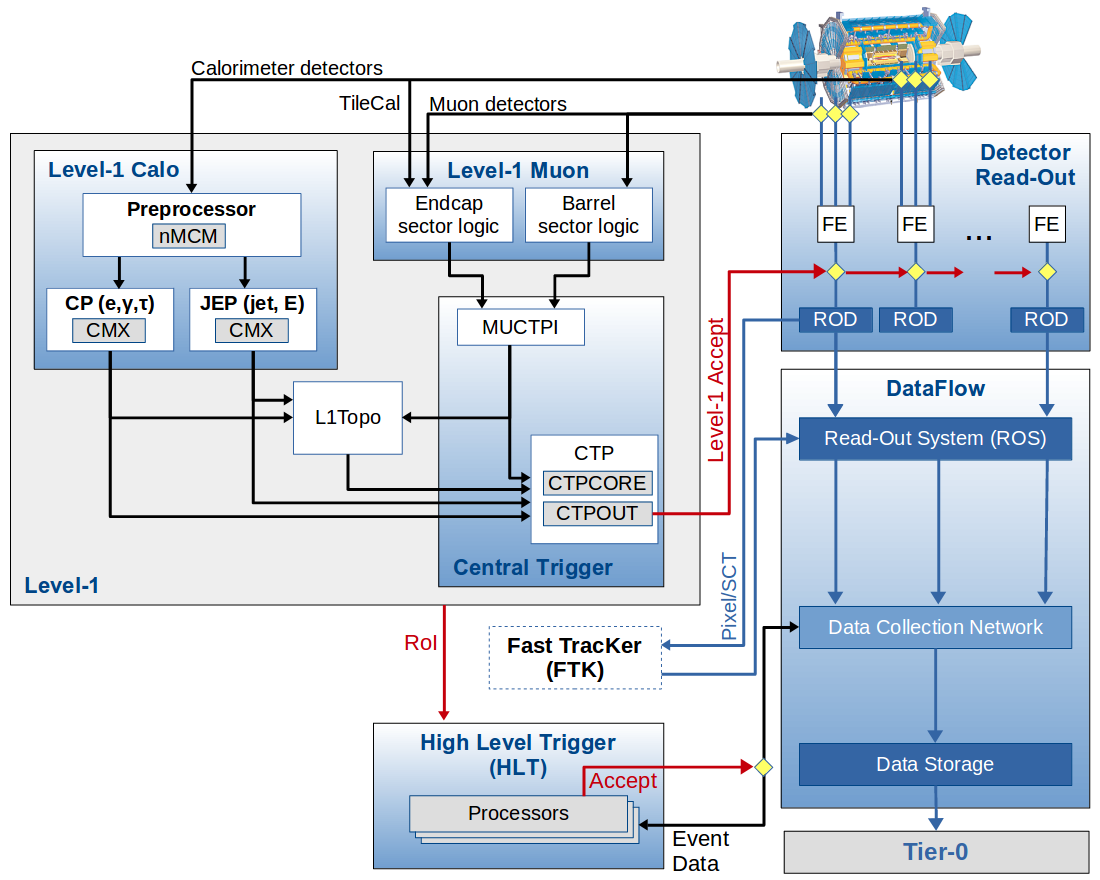
\includegraphics[width=.6\textwidth]{figures/Detector/tdaq-schematic.png}
\caption{A detailed schematic of the trigger and data acquisition infrastructure for Run 2. FTK was not a part of the Run 2 trigger system. \cite{TRIG-2016-01}}
\label{fig:tdaq-schematic}
\end{figure}


The \ac{L1} trigger has access to information from the calorimeters and the \ac{MS} \cite{TRIG-2016-01}. The \ac{ID} is not used at this stage due to the large number of readout channels as well as the computational intensity of track reconstruction. \ac{L1Calo} uses information from both calorimeters to identify electrons, photons, $\tau$ leptons, jets, and \ac{MET}. It divides the calorimeters into coarse-grained, $\Delta \eta \times \Delta \phi = 0.1 \times 0.1$ towers. Its algorithms look for towers with large deposits to define an \ac{RoI}. Based on the shape and size of the summed energy deposits around the tower, the cluster is classified. It then correlates these clusters across the event, to identify the number of candidates of a given physics object, and calculates \ac{MET}. \ac{L1Muon} looks for coincidences between different layers of the \ac{RPC} and \ac{TGC} detectors to identify hight \pt muons consistent with the interaction point. 

The decision to accept or reject an event at \ac{L1} is made by the \ac{CTP}, which uses a \emph{trigger menu} that describes which event topologies with which energies should be passed to the \ac{HLT}. If the event is accepted by the \ac{L1} trigger, full information from the whole detector is read out and passed to the \ac{HLT}. The \ac{HLT} also receives the location of the \acp{RoI}. An example of the \ac{L1} trigger rates in one run in September 2018 is shown in \autoref{fig:l1-rates}. About a third of events are selected as each an \ac{EM}, muon, or hadronic signature.

\begin{figure}[!h]
\centering
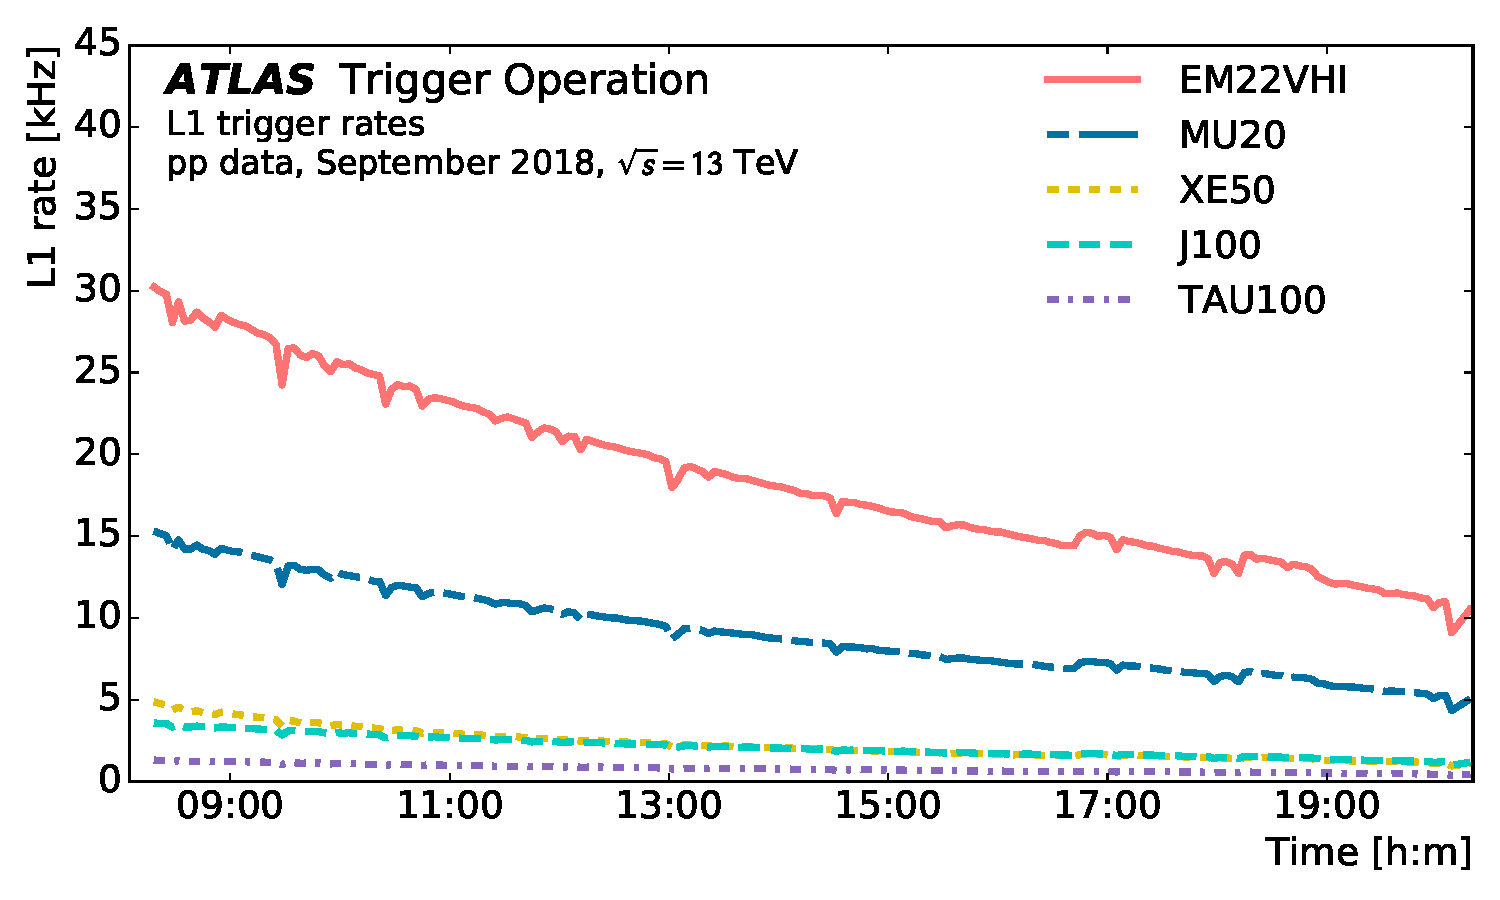
\includegraphics[width=.6\textwidth]{figures/Detector/l1-rates.pdf}
\caption{\ac{L1} trigger rates as a function of time in a fill taken in September 2018 with a peak luminosity of $L = 2.0 \times 10^{34}~\text{cm}^{-2}\text{s}^{-1}$ and a peak average number of interactions per crossing 56. Trigger items are based on electromagnetic clusters (EM), muon candidates (MU), jet candidates (J), missing transverse energy (XE) and tau candidates (TAU). Dips in the rate are due to dead-time and spikes are caused by detector noise. The rates increase periodically due to LHC luminosity re-optimizations \cite{trigger-public}}
\label{fig:l1-rates}
\end{figure}

The \ac{HLT} receives much less data and therefore has more time to make a decision. The \ac{HLT} has its own trigger menu with more complex topologies. Full event reconstruction cannot be performed in 200 ms, so each \ac{HLT} algorithm is seeded by an \ac{L1} trigger and tracking is performed in \acp{RoI} to refine the particle identification. Events selected by any of the \ac{HLT} algorithms are saved to disk for offline reconstruction, described in the next chapter. An example of the \ac{HLT} rates grouped by physical process in one run in September 2018 is shown in \autoref{fig:hlt-rates}. The trigger rates represent collaboration priorities. Most events include jets, but the jet triggers do not take the largest fraction of the trigger rate. In fact, jets must be very high \pt or in events with other physics objects in order to be selected. Large proportions of the \ac{HLT} rate is allocated to electrons and muons so that electroweak physics can be studied via events with leptonic W andZ boson decays. In general, single object triggers have very high \pt thresholds because they are more common, whereas multi-object triggers can select lower energy events while keeping the rate low.

\begin{figure}[!h]
\centering
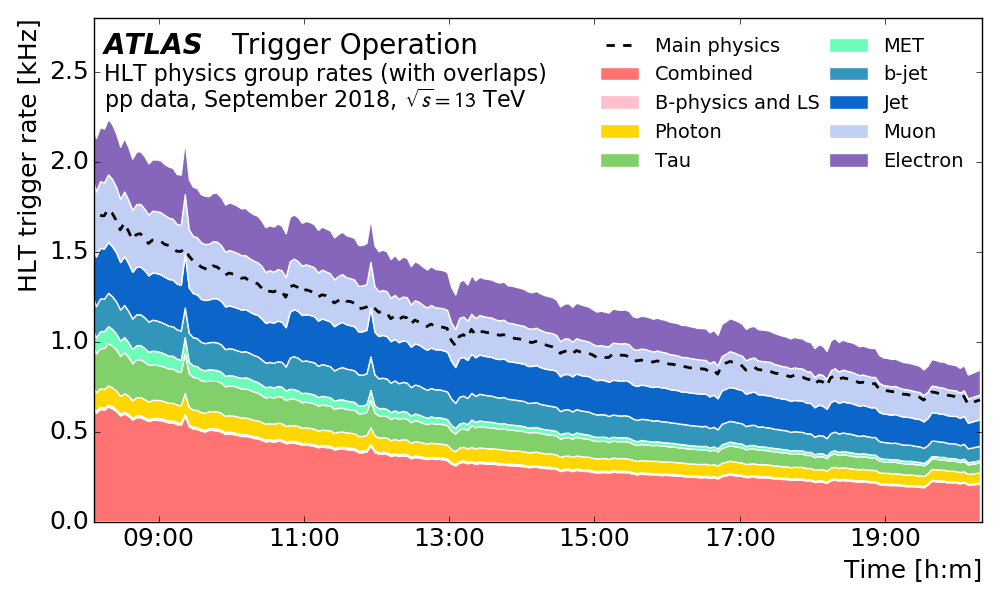
\includegraphics[width=.6\textwidth]{figures/Detector/hlt-rates.png}
\caption{\ac{HLT} trigger rates grouped by physics process as a function of time in a fill taken in September 2018 with a peak luminosity of $L = 2.0 \times 10^{34}~\text{cm}^{-2}\text{s}^{-1}$ and a peak average number of interactions per crossing 56. Each physics group contains single-object and multi-object triggers. The ``combined''combined represents triggers with multiple kinds of physics objects, like combinations of electrons, muons, taus, jets and \ac{MET}. All rates decrease exponentially with decreasing luminosity over the course of the fill.  Dips in the rate are due to dead-time and spikes are caused by detector noise. The rates increase periodically due to LHC luminosity re-optimizations  \cite{trigger-public}}
\label{fig:hlt-rates}
\end{figure}

Triggers are generally described by the physics object type and \pt threshold. Trigger rates can be limited by increasing the \pt threshold, or by making other selections on the object like limiting the $\eta$ range or requiring isolation. Triggers have some \emph{turn on} before they reach their peak efficiency, an example trigger is shown in \autoref{fig:hlt-electron}. \ac{HLT} triggers have higher energy thresholds than the \ac{L1} triggers to ensure the algorithms are being run where the previous trigger is fully efficient. Offline selections are similarly made above the energy thresholds of the \ac{HLT}.

\begin{figure}[!h]
\centering
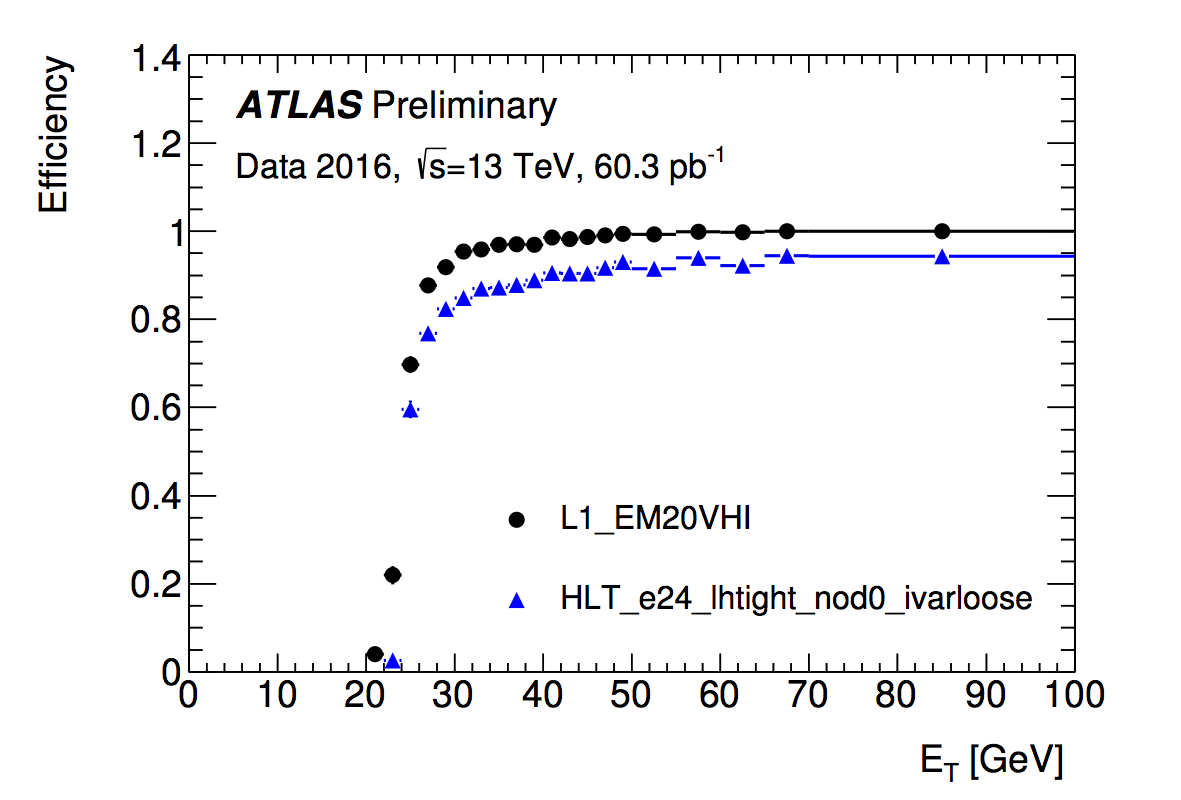
\includegraphics[width=.6\textwidth]{figures/Detector/hlt-electron.png}
\caption{An example of trigger efficiency as a function of transverse energy, \et, for a electron trigger. The \ac{L1} trigger is shown in black and the \ac{HLT} algorithm it seeded is shown in blue.  \cite{egamma-trigger-public}}
\label{fig:hlt-electron}
\end{figure}


\subsection{Triggers Used For This Analysis}

Nearly all searches for unconventional triggers face challenges finding a trigger. Tracking is only done in the \ac{HLT} near the \ac{L1} \acp{RoI}, so directly targeting peculiar tracks is challenging. Furthermore, the tracking done in the trigger assumes particles originate from the collision point and so electron and muon triggers veto displaced leptons whose tracks would not be reconstructed.

In order to avoid the dependence on tracking, \ac{MS}-signature-only triggers are used to identify displaced muons, and photon triggers (\ac{EM}-signature-only triggers) are used to identify displaced electrons. However, removing the tracking information removes an important discriminator from the \ac{HLT} algorithm, so these triggers suffer very high fake rates. Thus, they are otherwise limited. The muon trigger can only select muons with $|\eta| < 1.05$ and the single photon trigger has a high \pt threshold. The triggers used for this analysis are listed below and the requirements made on them in the analysis will be described in \autoref{sec:data}.

\begin{itemize}
	\item \texttt{HLT\_mu60\_0eta105\_msonly}
	\item \texttt{HLT\_g140\_loose}
	\item \texttt{HLT\_2g50\_loose}
\end{itemize}


These restrictions have particular effects on displaced leptons from \stau, particularly when the signature is one electron and one muon. The electron or muon result from a $\tau$ decay, not directly from the \stau decay, and thus have lower \pt. In order for an event to be selected, it must either have a muon in the narrow $\eta$ region, or a very high \pt electron, both of which are very unlikely. An \ac{HLT} algorithm has been designed for Run 3 that selects events with a photon and a \ac{MS} signature. The requirement of the two objects decreases the rate and allows for the $\eta$ and \pt thresholds to be relaxed. 



